\section{Experiments}
\label{sec:experiments}

\subsection{Setting}
\label{subsec:exp-setting}

For each \acs{drausp} benchmark instance, which are also used in the experiments of \textcite{drausp_lion18}, we train both the Standard-DQN baseline from
Section~\ref{sec:rl-approach} and the Lattice-DQN from Section~\ref{subsec:lattice-architecture}
using action masking, the target-network soft update, and the reject-biased $\epsilon$-greedy
exploration described earlier. To provide a fair comparision between the two networks, we adapt the layer sizes of the Standard-DQN to have the same number of parameters as the Lattice-DQN for each instance. 

\textbf{Parameters.} Unless noted otherwise, both networks are trained with the same
training-scheme parameters: reject-bias $\alpha=0.75$, $\gamma = 0.99$, $\epsilon$ decaying from
$1.0$ to $0.05$ over $T_d \cdot 1{.}000$ steps ($10{.}000$ for $T_d=10$, $20{.}000$ for $T_d=20$
and $50{.}000$ for $T_d=50$), a replay buffer of $50{.}000$ transitions with a $500$-step warm-up,
batch size $64$ and one training step every $4$ environment steps.

\textbf{Monotonicity test.} We evaluate the agents' monotonicity behavior every $100$ training
episodes by sampling $5$ trajectories, creating pairs of states as described in
Section~\ref{subsec:monotonicity-test}, and counting the number of monotonicity violations in
these pairs. This test is applied identically to both networks.

\textbf{Evaluation.} After performing $10{,}000$ training episodes, the agent's performance is evaluated; note that the network
weights do not change anymore here. We report the average performance on $10{,}000$ episodes with
$\epsilon = 0$. Monotonicity is evaluated by running the monotonicity tests for the different
parameters, each with $10{,}000$ pairs.

\textbf{Model comparison.} In Section~\ref{subsec:lattice-params} we determined the exact number
of parameters for the Lattice-DQN architecture dependent on the number of resources $K$,
calibrator keypoints $P$, and ensemble widths $U_1$ and $U_2$. We fix the number of calibrator keypoints $P=8$ and
the ensemble widths $U_1=4, U_2=2$, hence the number of parameters is only dependent on the number of resources
$K$. To obtain a fair comparison, we adapt the layer sizes of a two layer Standard-DQN to have the same
number of learnable parameters as the Lattice-DQN for each instance. We want to ensure by this that the model complexity is the same for both networks.


\subsection{Standard-DQN}
\label{subsec:exp-standard-dqn}

The Standard-DQN baseline is a standard two-layer feedforward network with no structural knowledge
of the monotonicity relations from Section~\ref{subsec:monotonicity}.

\textbf{Monotonicity behavior.} The standard DQN still manages to learn a policy that is mostly monotone, with only a few violations. Especially
the monotonicity in $C_k$ and the monotonicity in the mixed pairs is learned very well, and is fulfilled after few training episodes already.
Monotonicity in $t$ shows an interesting behavior: first the monotonicity drops to a ratio of $0.2$,
however during training the monotonicity recovers and gets to a perfect ratio of $1.0$ at the end. This behaviour can
be seen across different instances. 
The monotonicity in $q$ and $r$ is learned well from the beginning on and achieves a ratio $>0.8$ in the end. \\
An illustrative example of the training phase together with the monotonicity behavior is shown in Figure~\ref{fig:standard_dqn_training} for the benchmark instance SB05 with $T_d=50$.

\textbf{Performance.} After $4000$ episodes of training the agent's performance is already 
very good and a stable reward niveau is achieved. From this point on, the reward only increases slow and 
the $50$-episodes moving average fluctuates around the final reward.
The final evaluation phase shows that the agent achieves a very good performance, which is close to the optimal expected objective value $Z^*$ of the SDP formulation of \textcite{drausp_lion18}.
Remark that the result in the final evaluation is higher than in the training phase, which is due to the fact that the evaluation is performed with $\epsilon=0$ and therefore no random actions are taken.
\begin{figure}[ht]
	\centering
	\hspace*{-1.8cm}
	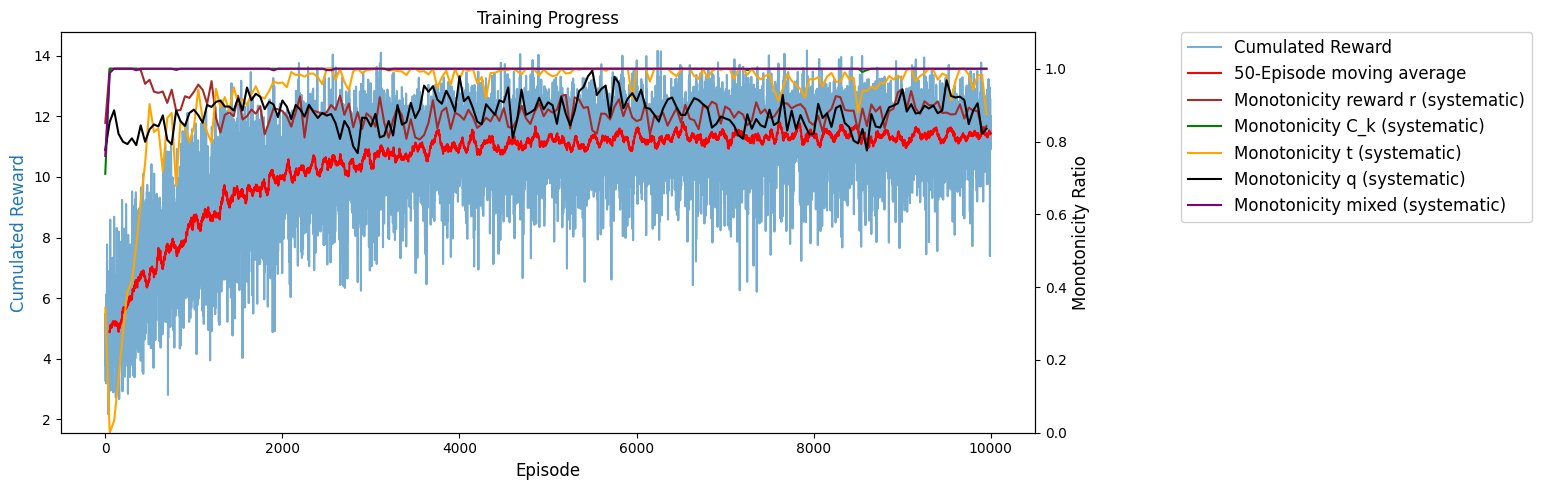
\includegraphics[scale=0.5]{grafiken/Experiments/standard_DQN_mono_SB5_all.png}
	\caption[Standard-DQN training and monotonicity behavior (SB05, $T_d=50$)]{Standard-DQN: training performance and monotonicity behavior on SB05, $T_d = 50$, over $10\,000$ training episodes.}
	\label{fig:standard_dqn_training}
\end{figure}
\begin{figure}[ht]
	\centering
	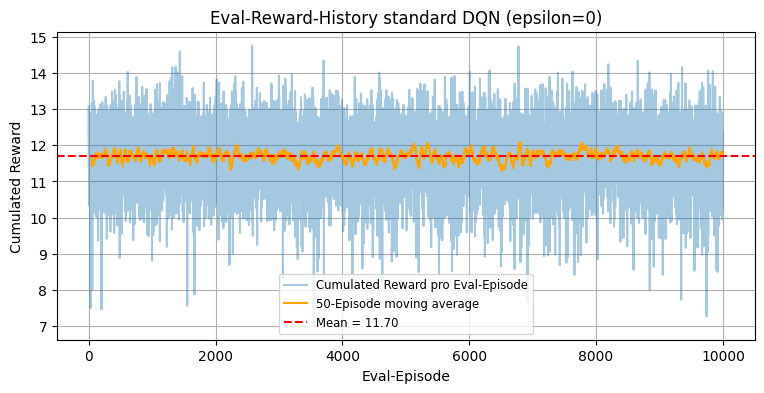
\includegraphics[scale=0.5]{grafiken/Experiments/standard_DQN_eval_SB5.png}
	\caption[Standard-DQN evaluation phase (SB05, $T_d=50$)]{Standard-DQN: evaluation phase on SB05, $T_d = 50$.}
	\label{fig:standard_dqn_eval}
\end{figure}

\subsection{Lattice-DQN}
\label{subsec:exp-lattice-dqn}

The Lattice-DQN is built up exactly as described in Section~\ref{subsec:lattice-architecture}.

\textbf{Monotonicity behavior.} Not surprisingly the monotonicity behavior is perfect from the
beginning on, as the network architecture enforces monotonicity by design. An example of the
training phase is shown in Figure~\ref{fig:lattice_dqn_training} for the benchmark instance SB05
with $T_d=50$.

\textbf{Performance.} Compared to a Standard-DQN with the same number of parameters, the agent has
to learn the same policy with a more constrained function class. This has to be taken into account
when designing the training architecture: the Lattice network needs considerably more fine-tuning
of the hyperparameters, whereas the Standard-DQN is much more robust to small changes in the
training-scheme hyperparameters (e.g.\ $\epsilon$-decay steps, reject bias, number of episodes).
Nevertheless, using the described training architecture in \ref{subsec:exp-setting}, the results are comparable
to the ones obtained by the standard \ac{dqn}. 

\begin{figure}[ht]
	\centering
	\hspace*{-1.8cm}
	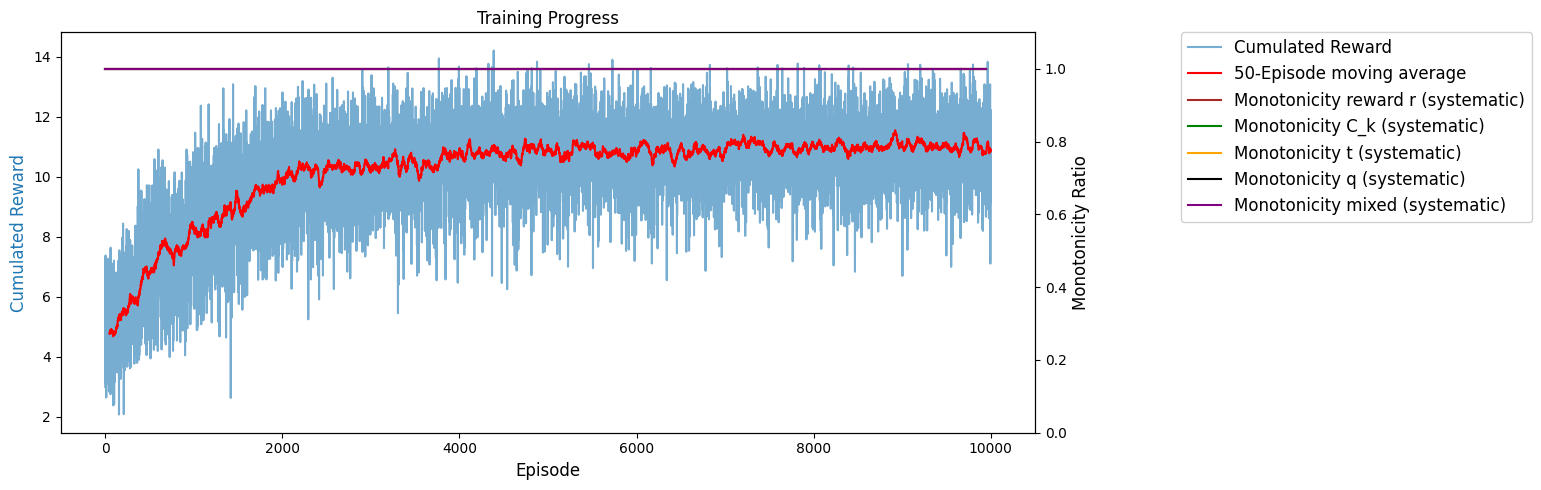
\includegraphics[scale=0.5]{grafiken/Experiments/Deep_Lattice_mono_SB5_all.png}
	\caption[Lattice-DQN training and monotonicity behavior (SB05, $T_d=50$)]{Lattice-DQN: training performance and monotonicity behavior on SB05, $T_d = 50$, over $10\,000$ training episodes.}
	\label{fig:lattice_dqn_training}
\end{figure}

\subsection{Numerical results}
\label{subsec:exp-results}

Tables~\ref{tab:results-s} and~\ref{tab:results-w} compare both agents against the optimal
expected objective value $Z^*$ of the SDP formulation of \textcite{drausp_lion18} (Table~1
and Table~2, respectively). $\bar R_{\text{eval}}$ is the mean cumulated reward over $10\,000$
evaluation episodes with $\epsilon = 0$, reported as mean $\pm$ one standard deviation across
those episodes. The monotonicity columns report the final ratio of
satisfied pairs ($10\,000$ pairs per axis) for the Standard-DQN; the Lattice-DQN satisfies every
check exactly by construction (ratio $1.00$ throughout) and is therefore omitted there. The
runtime columns are wall-clock seconds for the $10\,000$ training episodes and the $10\,000$
evaluation episodes, given as Standard-DQN\,/\,Lattice-DQN; entries marked $\dagger$ were
distorted by concurrent load on the shared machine and are not representative.

\begin{table}[htbp]
  \centering
  \footnotesize
  \setlength{\tabcolsep}{4pt}
  \caption[Results on the \texttt{lion18s} scheduling instances]{Results for the \texttt{lion18s} instances that require scheduling
    ($\text{len}(q) < K$; blocks \texttt{SA} $K=4$, \texttt{SB} $K=8$, \texttt{SC} $K=12$).
    $Z^*$ from \textcite{drausp_lion18}, Table~2.}
  \label{tab:results-s}
  \resizebox{\ifdim\width>\linewidth\linewidth\else\width\fi}{!}{%
  \begin{tabular}{l r r r r r r r r r r r}
    \toprule
     & & & \multicolumn{2}{c}{$\bar R_{\text{eval}} \pm s$} & \multicolumn{5}{c}{Monotonicity (Standard-DQN)} & \multicolumn{2}{c}{Runtime [s]} \\
    \cmidrule(lr){4-5}\cmidrule(lr){6-10}\cmidrule(lr){11-12}
    Instance & $T_d$ & $Z^*$ & DQN & Lat. & $C_k$ & $t$ & $r$ & $q_k$ & mix & train & eval \\
    \midrule
    SA01 & 10 & 5.08 & $5.08{\scriptstyle\,\pm\,0.85}$ & $5.03{\scriptstyle\,\pm\,0.86}$ & 0.99 & 1.00 & 0.90 & 0.84 & 1.00 & 266\,/\,2123 & 20\,/\,158 \\
    SA02 & 20 & 8.80 & $8.58{\scriptstyle\,\pm\,1.11}$ & $8.17{\scriptstyle\,\pm\,1.19}$ & 1.00 & 1.00 & 0.86 & 0.77 & 1.00 & 490\,/\,3387 & 39\,/\,295 \\
    SA03 & 50 & 13.44 & $13.10{\scriptstyle\,\pm\,1.10}$ & $12.39{\scriptstyle\,\pm\,1.03}$ & 1.00 & 0.74 & 0.82 & 0.84 & 1.00 & 1105\,/\,7403 & 92\,/\,1106 \\
    SA04 & 10 & 4.35 & $4.23{\scriptstyle\,\pm\,0.86}$ & $4.04{\scriptstyle\,\pm\,0.81}$ & 0.99 & 1.00 & 0.87 & 0.78 & 1.00 & 238\,/\,2494 & 19\,/\,262 \\
    SA05 & 20 & 5.97 & $5.87{\scriptstyle\,\pm\,0.69}$ & $4.49{\scriptstyle\,\pm\,0.79}$ & 1.00 & 0.96 & 0.82 & 0.80 & 1.00 & 447\,/\,3746 & 35\,/\,298 \\
    SA06 & 50 & 7.80 & $7.62{\scriptstyle\,\pm\,0.58}$ & $6.97{\scriptstyle\,\pm\,0.63}$ & 1.00 & 0.81 & 0.87 & 0.86 & 1.00 & 919\,/\,7374 & 78\,/\,802 \\
    SA07 & 10 & 5.08 & $5.06{\scriptstyle\,\pm\,0.85}$ & $5.09{\scriptstyle\,\pm\,0.84}$ & 1.00 & 1.00 & 0.96 & 0.77 & 1.00 & 255\,/\,39766$^{\dagger}$ & 20\,/\,269 \\
    SA08 & 20 & 10.16 & $10.16{\scriptstyle\,\pm\,1.18}$ & $10.08{\scriptstyle\,\pm\,1.23}$ & 1.00 & 1.00 & 0.91 & 0.83 & 1.00 & 539\,/\,4502 & 40\,/\,269 \\
    SA09 & 50 & 20.38 & $19.40{\scriptstyle\,\pm\,1.59}$ & $15.58{\scriptstyle\,\pm\,1.88}$ & 1.00 & 1.00 & 0.93 & 0.90 & 1.00 & 1214\,/\,7282 & 92\,/\,496 \\
    SA10 & 10 & 5.08 & $5.07{\scriptstyle\,\pm\,0.84}$ & $5.08{\scriptstyle\,\pm\,0.84}$ & 0.99 & 1.00 & 0.94 & 0.60 & 1.00 & 252\,/\,1825 & 21\,/\,138 \\
    SA11 & 20 & 9.02 & $8.47{\scriptstyle\,\pm\,1.03}$ & $8.17{\scriptstyle\,\pm\,1.25}$ & 1.00 & 1.00 & 0.87 & 0.77 & 1.00 & 490\,/\,3314 & 37\,/\,262 \\
    SA12 & 50 & 13.43 & $12.87{\scriptstyle\,\pm\,1.35}$ & $10.03{\scriptstyle\,\pm\,1.07}$ & 1.00 & 1.00 & 0.92 & 0.82 & 1.00 & 1102\,/\,6100 & 92\,/\,355 \\
    SA13 & 10 & 4.90 & $4.90{\scriptstyle\,\pm\,0.91}$ & $4.90{\scriptstyle\,\pm\,0.90}$ & 0.99 & 1.00 & 0.90 & 0.79 & 1.00 & 268\,/\,1818 & 20\,/\,134 \\
    SA14 & 20 & 8.79 & $8.55{\scriptstyle\,\pm\,1.12}$ & $8.27{\scriptstyle\,\pm\,1.24}$ & 1.00 & 1.00 & 0.96 & 0.80 & 1.00 & 494\,/\,3445 & 38\,/\,262 \\
    \addlinespace
    SB01 & 10 & 5.08 & $5.09{\scriptstyle\,\pm\,0.83}$ & $5.08{\scriptstyle\,\pm\,0.85}$ & 0.99 & 0.99 & 0.99 & 0.88 & 1.00 & 269\,/\,2672 & 21\,/\,289 \\
    SB02 & 20 & 10.16 & $10.04{\scriptstyle\,\pm\,1.23}$ & $10.03{\scriptstyle\,\pm\,1.23}$ & 0.98 & 1.00 & 0.96 & 0.88 & 1.00 & 543\,/\,65769$^{\dagger}$ & 42\,/\,4505$^{\dagger}$ \\
    SB03 & 10 & 5.08 & $5.03{\scriptstyle\,\pm\,0.87}$ & $5.03{\scriptstyle\,\pm\,0.87}$ & 0.99 & 1.00 & 0.87 & 0.87 & 1.00 & 269\,/\,2508 & 21\,/\,170 \\
    SB04 & 20 & 8.76 & $8.48{\scriptstyle\,\pm\,1.12}$ & $8.15{\scriptstyle\,\pm\,1.16}$ & 1.00 & 1.00 & 0.95 & 0.95 & 1.00 & 520\,/\,4655 & 39\,/\,329 \\
    SB05 & 50 & 12.60 & $12.05{\scriptstyle\,\pm\,0.87}$ & $7.77{\scriptstyle\,\pm\,1.49}$ & 1.00 & 0.96 & 0.88 & 0.85 & 1.00 & 1146\,/\,8399 & 92\,/\,474 \\
    SB06 & 10 & 4.44 & $4.25{\scriptstyle\,\pm\,0.73}$ & $4.15{\scriptstyle\,\pm\,0.76}$ & 1.00 & 0.99 & 0.81 & 0.81 & 1.00 & 252\,/\,2416 & 19\,/\,154 \\
    SB07 & 20 & 5.85 & $5.55{\scriptstyle\,\pm\,0.67}$ & $5.14{\scriptstyle\,\pm\,0.74}$ & 1.00 & 0.99 & 0.85 & 0.85 & 1.00 & 452\,/\,4223 & 35\,/\,254 \\
    SB08 & 50 & 7.53 & $7.00{\scriptstyle\,\pm\,0.55}$ & $6.18{\scriptstyle\,\pm\,0.81}$ & 1.00 & 0.62 & 0.85 & 0.78 & 1.00 & 966\,/\,8246 & 73\,/\,489 \\
    SB09 & 10 & 3.38 & $3.24{\scriptstyle\,\pm\,0.58}$ & $3.21{\scriptstyle\,\pm\,0.59}$ & 0.98 & 0.99 & 0.83 & 0.93 & 1.00 & 253\,/\,2552 & 20\,/\,163 \\
    SB10 & 20 & 4.28 & $3.90{\scriptstyle\,\pm\,0.52}$ & $4.02{\scriptstyle\,\pm\,0.54}$ & 0.98 & 0.95 & 0.87 & 0.85 & 1.00 & 487\,/\,4678 & 35\,/\,308 \\
    \addlinespace
    SC01 &  5 & 2.54 & $2.50{\scriptstyle\,\pm\,0.60}$ & $2.50{\scriptstyle\,\pm\,0.60}$ & 0.99 & 1.00 & 0.98 & 0.90 & 1.00 & 141\,/\,1659 & 11\,/\,94 \\
    SC02 &  5 & 2.32 & $2.22{\scriptstyle\,\pm\,0.57}$ & $2.23{\scriptstyle\,\pm\,0.58}$ & 0.98 & 0.98 & 0.96 & 0.74 & 1.00 & 141\,/\,1615 & 11\,/\,89 \\
    SC03 &  5 & 1.74 & $1.68{\scriptstyle\,\pm\,0.40}$ & $1.61{\scriptstyle\,\pm\,0.40}$ & 0.98 & 0.97 & 0.86 & 0.87 & 1.00 & 126\,/\,1454 & 9\,/\,80 \\
    SC04 & 10 & 2.17 & $2.04{\scriptstyle\,\pm\,0.37}$ & $2.06{\scriptstyle\,\pm\,0.38}$ & 0.99 & 0.97 & 0.91 & 0.91 & 1.00 & 225\,/\,2648 & 16\,/\,154 \\
    SC05 & 20 & 2.55 & $2.40{\scriptstyle\,\pm\,0.31}$ & $2.29{\scriptstyle\,\pm\,0.35}$ & 0.97 & 0.94 & 0.89 & 0.82 & 1.00 & 412\,/\,4365 & 30\,/\,264 \\
    \bottomrule
  \end{tabular}%
  }
\end{table}

\begin{table}[htbp]
  \centering
  \footnotesize
  \setlength{\tabcolsep}{4pt}
  \caption[Results on the \texttt{lion18w} accept/reject instances]{Results for the \texttt{W} instances (\texttt{lion18w}; blocks \texttt{WA} $K=4$,
    \texttt{WB} $K=8$, \texttt{WC} $K=12$, all with $\text{len}(q) = K$, i.e.\ accept/reject only).
    $Z^*$ from \textcite{drausp_lion18}, Table~1.}
  \label{tab:results-w}
  \resizebox{\ifdim\width>\linewidth\linewidth\else\width\fi}{!}{%
  \begin{tabular}{l r r r r r r r r r r r}
    \toprule
     & & & \multicolumn{2}{c}{$\bar R_{\text{eval}} \pm s$} & \multicolumn{5}{c}{Monotonicity (Standard-DQN)} & \multicolumn{2}{c}{Runtime [s]} \\
    \cmidrule(lr){4-5}\cmidrule(lr){6-10}\cmidrule(lr){11-12}
    Instance & $T_d$ & $Z^*$ & DQN & Lat. & $C_k$ & $t$ & $r$ & $q_k$ & mix & train & eval \\
    \midrule
    WA01 & 10 & 4.33 & $4.25{\scriptstyle\,\pm\,0.84}$ & $4.13{\scriptstyle\,\pm\,0.87}$ & 0.99 & 1.00 & 0.82 & 0.62 & 1.00 & 244\,/\,1900 & 19\,/\,153 \\
    WA02 & 20 & 6.43 & $6.11{\scriptstyle\,\pm\,0.99}$ & $5.81{\scriptstyle\,\pm\,1.04}$ & 0.99 & 0.98 & 0.65 & 0.78 & 1.00 & 457\,/\,3181 & 37\,/\,268 \\
    WA03 & 50 & 9.49 & $8.65{\scriptstyle\,\pm\,1.14}$ & $7.78{\scriptstyle\,\pm\,1.48}$ & 1.00 & 0.98 & 0.73 & 0.60 & 1.00 & 1046\,/\,5694 & 91\,/\,564 \\
    WA04 & 10 & 5.07 & $5.08{\scriptstyle\,\pm\,0.84}$ & $5.07{\scriptstyle\,\pm\,0.85}$ & 1.00 & 1.00 & 0.79 & 0.52 & 1.00 & 250\,/\,1962 & 20\,/\,167 \\
    WA05 & 20 & 9.23 & $9.09{\scriptstyle\,\pm\,1.20}$ & $8.24{\scriptstyle\,\pm\,1.60}$ & 1.00 & 1.00 & 0.79 & 0.64 & 1.00 & 491\,/\,3385 & 38\,/\,284 \\
    WA06 & 50 & 15.36 & $14.44{\scriptstyle\,\pm\,1.43}$ & $9.07{\scriptstyle\,\pm\,1.83}$ & 1.00 & 0.99 & 0.84 & 0.75 & 1.00 & 1144\,/\,5649 & 90\,/\,320 \\
    WA07 & 10 & 4.35 & $4.29{\scriptstyle\,\pm\,0.88}$ & $3.99{\scriptstyle\,\pm\,0.99}$ & 0.98 & 1.00 & 0.85 & 0.60 & 1.00 & 247\,/\,1766 & 19\,/\,144 \\
    WA08 & 20 & 6.58 & $6.35{\scriptstyle\,\pm\,1.05}$ & $5.58{\scriptstyle\,\pm\,1.23}$ & 1.00 & 0.99 & 0.83 & 0.73 & 1.00 & 460\,/\,3179 & 37\,/\,250 \\
    \addlinespace
    WB01 & 10 & 4.08 & $3.94{\scriptstyle\,\pm\,0.74}$ & $3.89{\scriptstyle\,\pm\,0.76}$ & 0.99 & 1.00 & 0.84 & 0.70 & 1.00 & 242\,/\,2346 & 18\,/\,151 \\
    WB02 & 20 & 5.47 & $5.08{\scriptstyle\,\pm\,0.71}$ & $4.90{\scriptstyle\,\pm\,0.78}$ & 0.99 & 0.98 & 0.75 & 0.75 & 1.00 & 440\,/\,3946 & 34\,/\,250 \\
    WB03 & 50 & 7.19 & $6.69{\scriptstyle\,\pm\,0.73}$ & $5.68{\scriptstyle\,\pm\,0.82}$ & 1.00 & 0.99 & 0.81 & 0.86 & 1.00 & 891\,/\,6760 & 83\,/\,489 \\
    WB04 & 10 & 1.69 & $1.67{\scriptstyle\,\pm\,0.43}$ & $1.66{\scriptstyle\,\pm\,0.42}$ & 0.97 & 0.96 & 0.69 & 0.77 & 1.00 & 215\,/\,2140 & 18\,/\,147 \\
    WB05 & 20 & 2.08 & $2.01{\scriptstyle\,\pm\,0.43}$ & $1.93{\scriptstyle\,\pm\,0.44}$ & 0.98 & 0.96 & 0.69 & 0.72 & 1.00 & 434\,/\,3767 & 31\,/\,248 \\
    WB06 & 10 & 3.22 & $3.17{\scriptstyle\,\pm\,0.59}$ & $3.11{\scriptstyle\,\pm\,0.61}$ & 0.98 & 0.99 & 0.86 & 0.74 & 1.00 & 239\,/\,2335 & 19\,/\,160 \\
    WB07 & 20 & 4.06 & $3.94{\scriptstyle\,\pm\,0.57}$ & $3.58{\scriptstyle\,\pm\,0.59}$ & 0.98 & 0.99 & 0.72 & 0.80 & 1.00 & 460\,/\,4480 & 35\,/\,248 \\
    \addlinespace
    WC01 & 10 & 1.54 & $1.52{\scriptstyle\,\pm\,0.30}$ & $1.48{\scriptstyle\,\pm\,0.29}$ & 0.99 & 0.95 & 0.79 & 0.79 & 0.99 & 223\,/\,2629 & 17\,/\,139 \\
    WC02 & 20 & 1.78 & $1.75{\scriptstyle\,\pm\,0.28}$ & $1.71{\scriptstyle\,\pm\,0.25}$ & 1.00 & 0.96 & 0.72 & 0.69 & 0.96 & 400\,/\,4663 & 30\,/\,245 \\
    WC03 & 50 & 2.13 & $2.02{\scriptstyle\,\pm\,0.30}$ & $1.60{\scriptstyle\,\pm\,0.31}$ & 1.00 & 0.90 & 0.82 & 0.46 & 0.98 & 851\,/\,9007 & 64\,/\,405 \\
    WC04 & 10 & 1.53 & $1.52{\scriptstyle\,\pm\,0.35}$ & $1.48{\scriptstyle\,\pm\,0.35}$ & 0.99 & 0.96 & 0.65 & 0.57 & 0.99 & 228\,/\,2670 & 17\,/\,146 \\
    WC05 & 20 & 1.79 & $1.73{\scriptstyle\,\pm\,0.30}$ & $1.72{\scriptstyle\,\pm\,0.30}$ & 0.98 & 0.95 & 0.82 & 0.91 & 1.00 & 412\,/\,4560 & 29\,/\,271 \\
    WC06 & 50 & 2.17 & $1.92{\scriptstyle\,\pm\,0.34}$ & $1.88{\scriptstyle\,\pm\,0.32}$ & 1.00 & 0.78 & 0.38 & 0.66 & 1.00 & 890\,/\,8836 & 58\,/\,483 \\
    \bottomrule
  \end{tabular}%
  }
\end{table}

The Standard-DQN reaches $90$--$100\%$ of $Z^*$ on almost all instances and is at or above the
Lattice-DQN in evaluation reward essentially everywhere. The Lattice-DQN matches it on the easy
instances but falls off markedly on the harder large-$T_d$ cases, where its more constrained
function class limits the attainable policy: e.g.\ SB05 ($7.77$ vs.\ $12.05$, $62\%$ of $Z^*$),
SA09 ($15.58$ vs.\ $19.40$), WA06 ($9.07$ vs.\ $14.44$) and WC03 ($1.60$ vs.\ $2.02$). The
Standard-DQN learns monotonicity in $C_k$, $t$ and the mixed pairs almost perfectly, but only
partially in $r$ and especially $q_k$, which drops below $0.6$ on some instances (SA10, WA04,
WC03). Training the Lattice-DQN takes roughly $5$--$12\times$ longer than the parameter-matched
Standard-DQN, caused by the per-step constraint projection and the many small lattice
evaluations.
